\section{Aufbau und Durchführung}
\label{sec:Durchführung}

\subsection{Aufbau}
Der Aufbau des Versuchs ist in Abbildung \ref{fig:aufbau} zu sehen. Die wesentlichen
Elemente sind die Kupfer-Röntgenröhre, ein LiF-Kristall sowie ein Geiger-Müller-Zählrohr.
Die Kupfer-Röntgenröhre liefert die Röntgenstrahlung. Sie wird fokussiert auf den Kristall
gelenkt und dort unter den Bestimmungen der Bragg'schen Bedingung reflektiert. Dann
treffen die Photonen auf ein Geiger-Müller-Zählrohr, das die Intensität aufnimmt.
Am Geiger-Müller-Zählrohr ist vorne eine Schlitzblende angebracht, die waagerecht ausgerichtet
ist um nicht Strahlen unterschiedlicher Wellenlängen aufzuzeichnen.
Dieser Aufbau ist an einen Computer angeschlossen, der den Kristall und das Geiger-Müller-Zählrohr
relativ zum Strahl drehen kann. So kann die Intensität in Abhängigkeit zum Winkel
aufgenommen werden. Der Computer nimmt dann auch die Messdaten auf.

\begin{figure}
  \centering
  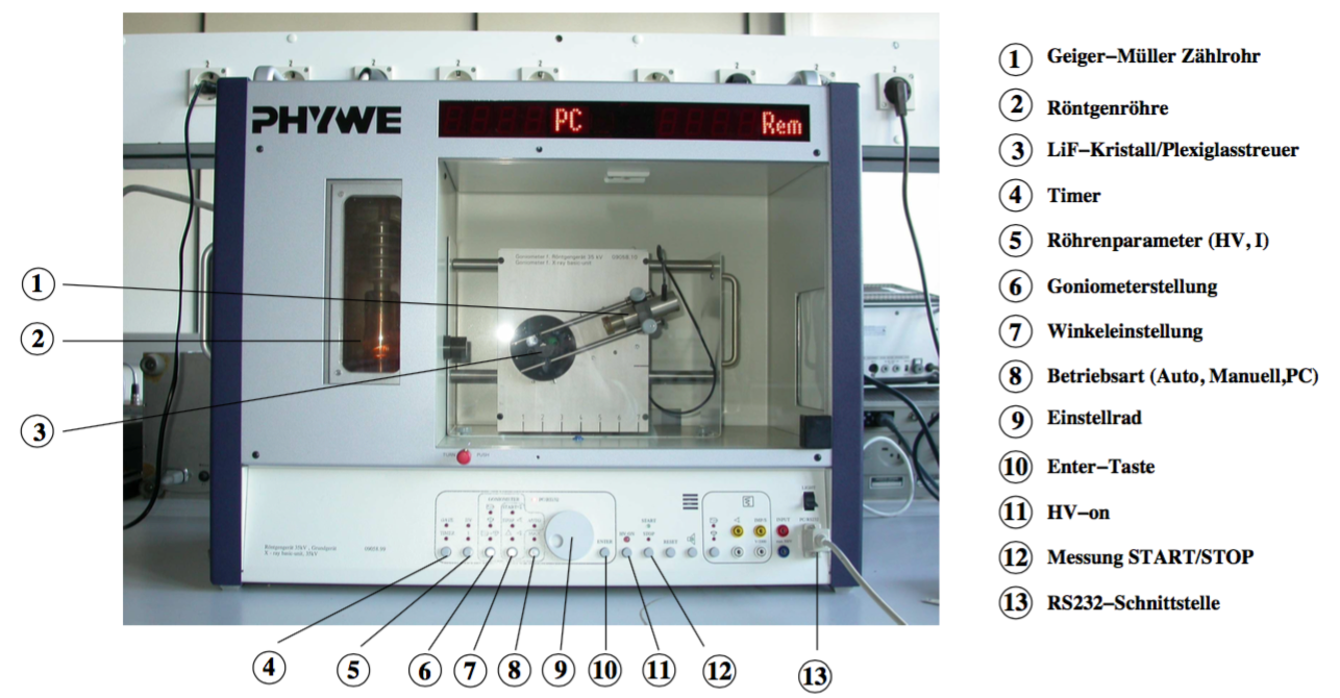
\includegraphics[width = \textwidth]{Pics/Aufbau.pdf}
  \caption{Das Röntgengerät bestehend aus vielen Bauteilen. \cite{anleitung}}
  \label{fig:aufbau}
\end{figure}

\subsection{Durchführung}

Bei allen Messungen sollte die Beschleunigungsspannung auf
$U_{\g{B}} = \SI{35}{\kilo\volt}$ und der Emissionsstrom auf $I = \SI{1}{\milli\ampere}$
eingestellt sein.

\subsubsection{Überprüfung der Bragg Bedingung}

Hier wird der Kristallwinkel auf feste $\SI{14}{\degree}$ gestellt und mit dem
Geiger-Müllerzählrohr der Winkelbereich von $\alpha_{\g{GM}} = \SI{26}{\degree}$
bis $\alpha_{\g{GM}} = \SI{30}{\degree}$ mit einem Winkelzuwachs von
$\Delta \alpha = \SI{0.1}{\degree}$ abgefahren. Die Intergrationszeit beträgt
$\Delta t = \SI{5}{\second}$. Das Maximum der Kurve wird bei $\SI{28}{\degree}$
erwartet, da dann der Glanzwinkel von $\SI{14}{\degree}$ relativ zum Kristall erreicht ist.

\subsubsection{Emissionsspektrum der Kupfer-Röntgenröhre}

Zur Aufnahme des Emissionsspektrums wird am PC der \emph{2:1 Koppelmodus} gewählt.
Der Winkelbereich liegt hier bei $\SI{4}{\degree} \leq \theta \leq \SI{26}{\degree}$
und wird in $\SI{0.2}{\degree}$-Schritten mit einer Integrationszeit von $\Delta t = \SI{5}{\second}$
abgetastet.

\subsubsection{Das Absorptionsspektrum}

Für die Aufnahme des Absorptionsspektrums muss zunächst der Winkel berechnet werden, bei
dem die Absorptionskante erwartet wird. Dieser ist bei jedem Absorber verschieden.
Dann wird in einem circa $\SI{6}{\degree}$ großen Intervall mit einer Integrationszeit
von $\Delta t = \SI{20}{\second}$ und einem Winkelzuwachs von $\Delta \alpha = \SI{0.1}{\degree}$
um den Winkel herum gemessen. Die Absorber werden direkt vor das Zählrohr geschraubt.

Benutzt werden Germanium, Brom, Zirkonium und Bismuth als Absorber. Wobei bei der
Bestimmung des Winkels für Bismuth darauf geachtet werden muss, dass hier die
Abschirmkonstante $\sigma_{\g{L}}$ bestimmt wird.
